\documentclass[11pt]{amsart}

\usepackage{amsmath}
\usepackage{amssymb}
\usepackage{tikz}
\usepackage{pgfplots}
\usepackage{xcolor}

\DeclareMathOperator\erf{erf}

\newcommand{\airgrid}{\mathrm{air-grid}}
\newcommand{\app}{a}
\newcommand{\cutin}{\mathrm{cut-in}}
\newcommand{\cutout}{\mathrm{cut-out}}
\newcommand{\extra}{\mathrm{extra}}
\newcommand{\grav}{\mathrm{grav}}
\newcommand{\groundinverter}{\mathrm{ground\;inv.}}
\newcommand{\kiteinverter}{\mathrm{kite\;inv.}}
\newcommand{\kite}{k}
\newcommand{\lp}{\mathrm{loop}}
%\newcommand{\max}{\mathrm{max}}
\newcommand{\motor}{\mathrm{motor}}
\newcommand{\path}{\mathrm{path}}
\newcommand{\prop}{\mathrm{prop}}
\newcommand{\swept}{\mathrm{swept}}
\newcommand{\sys}{\mathrm{sys}}
\newcommand{\tether}{\mathrm{tether}}
\newcommand{\wind}{w}

\definecolor{matlab1}{rgb}{0, 0.4470, 0.7410}
\definecolor{matlab2}{rgb}{0.8500, 0.3250, 0.0980}
\definecolor{matlab3}{rgb}{0.9290, 0.6940, 0.1250}
\definecolor{matlab4}{rgb}{0.4940, 0.1840, 0.5560}
\definecolor{matlab5}{rgb}{0.4660, 0.6740, 0.1880}
\definecolor{matlab6}{rgb}{0.3010, 0.7450, 0.9330}
\definecolor{matlab7}{rgb}{0.6350, 0.0780, 0.1840}

\title{Crosswind kite power curve}
\author{Makani Technologies LLC}
\date{June 28, 2016}

\begin{document}
\maketitle

\section{Fundamentals}
\label{sec:fundamentals}

Traditional wind turbines use the power coefficient, $C_P$, as a
critical performance metric:
%
\begin{equation}
C_P = \frac{P}{\frac{1}{2} \rho v_{\wind}^3 A_{\swept}}
\end{equation}
%
This is the value that is optimized in the celebrated Betz limit,
which says that the maximum achievable power coefficient is $C_P \approx 0.593$.
Notably the power coefficient is referenced to the {\it swept area} of
the wind turbine blades, which is reasonable given the limited swept
area available to a traditional wind turbine.

For kite based systems, where system cost is correlated with kite size
rather than the vast swept area, it makes sense to reference the power
coefficient to {\it kite area}.  This value is referred to as $\zeta$:
%
\begin{equation}
\label{eqn:zeta}
\zeta = \frac{P}{\frac{1}{2} \rho v_{\wind}^3 A_{\kite}}
\end{equation}

However, optimizing a system for the maximum $C_P$ or $\zeta$ is not
the same as optimizing for cost!  In fact, optimizing a system for
maximum $\zeta$ actually increases the maximum tension, a substantial
cost driver, over a Betz limited system by a factor of two.  To
describe how efficiently a system converts tension into power, it is
useful to introduce another dimensionless variable, the tension
efficiency, $\eta_T$:
%
\begin{equation}
\label{eqn:eta_T}
\eta_T = \frac{P}{T v_{\wind}}
\end{equation}
%
According to actuator disk theory, for a Betz limited system, the wind
velocity at the disk, where it may be assumed the force is applied, is
$\frac{2}{3} v_{\wind}$.  Thus, the tension efficiency for a Betz
limited system is $\eta_T = \frac{2}{3}$.

To calculate the corresponding tension efficiency for a kite power
system that attempts to maximize $\zeta$, i.e. a Loyd limited system,
it is first necessary to relate $\zeta$ to physical properties of the
kite.  Ignoring power efficiency losses and the typically low
induction factors of kite propellers, the power generated by the kite
is approximately, $P = D_{\prop} v_{\kite}$, where $D_{\prop}$ is the
drag on all the propellers and $v_{\kite}$ is the airspeed of the
kite.  Substituting this into Eq. \ref{eqn:zeta}, it is found that
%
\begin{equation}
\label{eqn:zeta_prop}
\zeta = C_{D_{\prop}} \left(\frac{v_{\kite}}{v_{\wind}} \right)^3
\end{equation}

The kite-to-wind speed ratio, which figures prominently in
Eq. \ref{eqn:zeta_prop}, may be related to the lift and drag
coefficients of the kite through simple force balance.  Specifically,
the airspeed of a kite traveling perpendicular to the wind is given
by:
%
\begin{equation}
\label{eqn:kite_speed}
v_{\kite} = \sqrt{1 + \left(\frac{C_L}{C_D}\right)^2} v_{\wind}
          \approx \frac{C_L}{C_D} v_{\wind}
\end{equation}
%
Here the drag coefficient, $C_D$, may be divided into two components:
system drag, $C_{D_{\sys}}$, and propeller drag, $C_{D_{\prop}}$.  The
system drag coefficient includes parasitic drag, induced drag, and
tether drag, and to a large degree is fixed during flight.  The
propeller drag coefficient, however, may be tuned over a wide range.

To optimize propeller drag for various metrics, e.g. $\zeta$ or
$\eta_T$, it is useful to express the tunable propeller drag
coefficient as a fraction, $k$, of the fixed system drag coefficient:
$C_{D_{\prop}} = k C_{D_{\sys}}$.  Now, the kite-to-wind speed ratio,
$\lambda$, from Eq. \ref{eqn:kite_speed} is
%
\begin{equation}
\label{eqn:lambda}
\lambda = \frac{v_{\kite}}{v_{\wind}} = \frac{C_L}{C_{D_{\sys}}} \frac{1}{1 + k}
\end{equation}
%
Thus, $\zeta$ from Eq. \ref{eqn:zeta_prop} is
%
\begin{equation}
\zeta = \frac{C_L^3}{C_{D_{\sys}}^2} \frac{k}{(1+k)^3}
\end{equation}
%
And finally, using the approximation for tension,
$T = \frac{1}{2} \rho v_{\kite}^2 A_{\kite} C_L$, the tension efficiency, $\eta_T$,
from Eq. \ref{eqn:eta_T}, is
%
\begin{equation}
\eta_T = \frac{k}{1 + k}
\end{equation}

\begin{figure}
\begin{center}
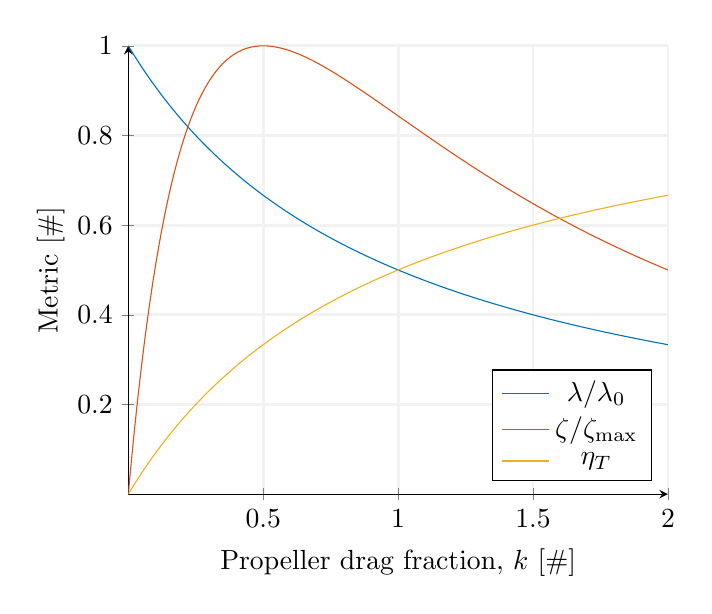
\begin{tikzpicture}
\begin{axis}[axis lines=middle, samples=200,
    grid=both,
    grid style={line width=1pt, draw=gray!10},
    x label style={at={(axis description cs:0.5,-0.1)}, anchor=north},
    y label style={at={(axis description cs:-0.1,.5)}, rotate=90, anchor=south},
    xlabel={Propeller drag fraction, $k$ [\#]},
    ylabel={Metric [\#]},
    legend pos=south east]
\addplot[matlab1, domain=0:2] {1 / (1 + x)};
\addplot[matlab2, domain=0:2] {x / (1 + x)^3 / (4/27)};
\addplot[matlab3, domain=0:2] {x / (1 + x)};
\legend{$\lambda / \lambda_0$, $\zeta / \zeta_{\max}$, $\eta_T$};
\end{axis}
\end{tikzpicture}
\caption{Kite performance metrics as a function of the propeller drag
  fraction.}
\end{center}
\end{figure}

There are many interesting things to note from the three dimensionless
performance metrics described above ($\lambda$, $\zeta$, and $\eta_T$):
\begin{itemize}
\item The kite speed is proportional to the system's
  lift-to-drag ratio, as expected, and this is tunable with the
  propeller drag.

\item The $C_L^3$ in the $\zeta$ metric really encourages high lift
  coefficients.  This effect is even more dramatic considering the
  high drag penalty imposed by the tether, which makes the increase in
  induced drag with $C_L^2$ less important when compared to other
  systems that optimize for the endurance metric.

\item Maximizing $\zeta$ requires setting the propeller drag to half
  the system drag, $k = \frac{1}{2}$.  From Eq. \ref{eqn:lambda}, this
  is equivalent to saying that the kite should fly at $\frac{2}{3}$ of
  its zero-propeller-drag speed.

\item The tension efficiency is independent of any system parameter
  save the propeller drag fraction.

\item Finally, optimizing for $\zeta$ results in a tension efficiency
  of $\eta_T = \frac{1}{3}$.  Thus, maximizing $\zeta$ results in half
  the tension efficiency of a Betz limited system.  Of course, it is
  not necessary to fly a system at maximum $\zeta$; and if $k$ is
  increased to 2, the system will achieve the same tension efficiency
  as a Betz limited device, but $\zeta$ will drop by a factor of 2.
\end{itemize}


\section{Ideal power curve}

\begin{figure}[h]
\label{fig:power_curve}
\begin{center}
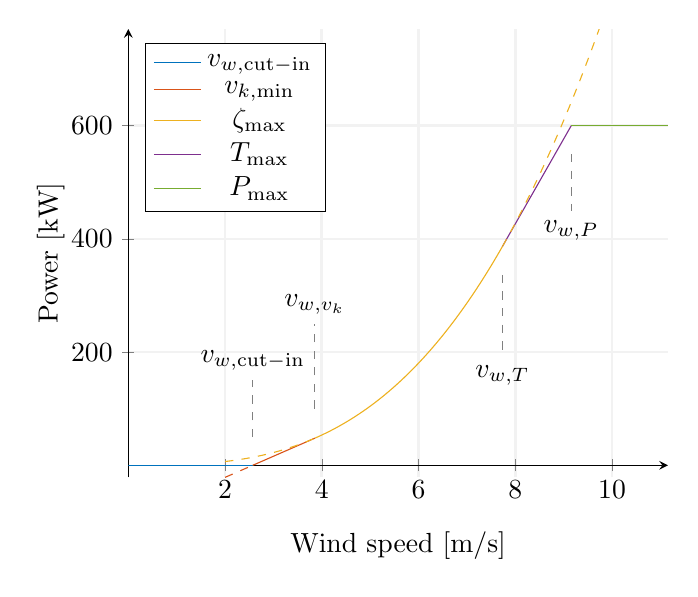
\begin{tikzpicture}
  \def\CL{2.1};
  \def\CDsys{0.18};
  \def\costheta{1};
  \def\etaairgrid{1};
  \def\Tmax{150};  % [kN]
  \def\Pmax{600};  % [kW]
  \def\zetamax{(4/27 * \CL^3 / \CDsys^2)};
  \def\Ak{32.9};
  \def\rho{1.2};
  \def\vkitemin{30};
  \def\P0{(0.5 * \rho * \Ak * \CDsys * \vkitemin^3 / 1000)};
  \def\vcutin{(\CDsys / \CL * \vkitemin / \costheta)};
  \def\vT{((\Tmax * 1000 / 3 / (0.5 * \rho * \Ak * \zetamax))^0.5 / \costheta)};
  \def\vP{(\Pmax / (\etaairgrid * \Tmax * \costheta) + 2 * \vT / 3)};
  \def\loydcoeff{(\etaairgrid * \costheta^3 * 0.5 * \rho * \Ak * \zetamax / 1000)};

\begin{axis}[axis lines=middle, samples=200,
    grid=both,
    grid style={line width=1pt, draw=gray!10},
    x label style={at={(axis description cs:0.5,-0.1)}, anchor=north},
    y label style={at={(axis description cs:-0.1,.5)}, rotate=90, anchor=south},
    xlabel={Wind speed [m/s]},
    ylabel={Power [kW]},
    legend pos=north west]
  \addplot[matlab1, domain=0:(\vcutin)] {0};
  \addplot[matlab2, domain=(\vcutin):(1.5 * \vcutin)] {\etaairgrid * \P0 * (x / \vcutin - 1)};
  \addplot[matlab3, domain=(1.5 * \vcutin):(\vT)] {\loydcoeff * x^3};
  \addplot[matlab4, domain=(\vT):(\vP)] {\etaairgrid * \costheta * \Tmax * (x - 2 * \vT / 3)};
  \addplot[matlab5, domain=(\vP):(\vP + 2)] {\Pmax};
  \legend{$v_{\wind,\cutin}$, $v_{\kite,\min}$, $\zeta_{\max}$, $T_{\max}$, $P_{\max}$};

  \addplot[matlab3, dashed, domain=2:(1.5 * \vcutin)] {\loydcoeff * x^3};
  \addplot[matlab3, dashed, domain=(\vT):(\vT + 2)] {\loydcoeff * x^3};
  \addplot[matlab2, dashed, domain=2:(\vcutin)] {\etaairgrid * \P0 * (x / \vcutin - 1)};

  \draw[gray, dashed] (axis cs:{\vcutin}, 50) -- (axis cs:{\vcutin}, 150)
  node [above, black] {$v_{\wind,\cutin}$};
  \draw[gray, dashed] (axis cs:{1.5 * \vcutin}, 100) -- (axis cs:{1.5 * \vcutin}, 250)
  node [above, black] {$v_{\wind,v_{\kite}}$};
  \draw[gray, dashed] (axis cs:{\vT}, {\loydcoeff * \vT^3 - 50}) -- (axis cs:{\vT}, {\loydcoeff * \vT^3 / 2})
  node [below, black] {$v_{\wind,T}$};
  \draw[gray, dashed] (axis cs:{\vP}, 550) -- (axis cs:{\vP}, 450)
  node [below, black] {$v_{\wind,P}$};

\end{axis}
\end{tikzpicture}
\caption{Representative ideal power curve showing the
  airspeed-limited, Loyd-limited, tension-limited, and power-limited
  segments.  This particular power curve assumes: $A_{\kite} = 32.9$
  m$^2$, $v_{\kite,\min} = 30$ m/s, $\zeta_{\max} = 42.3$, $T_{\max} = 150$
  kN, $P_0 = 96$ kW, and $P_{\max} = 600$ kW.}
\end{center}
\end{figure}

%% \begin{figure}
%% \label{fig:power_curve}
%% \begin{center}
%% \begin{tikzpicture}
%% \begin{axis}[axis lines=middle, samples=200,
%%     grid=both,
%%     grid style={line width=1pt, draw=gray!10},
%%     x label style={at={(axis description cs:0.5,-0.1)}, anchor=north},
%%     y label style={at={(axis description cs:-0.1,.5)}, rotate=90, anchor=south},
%%     xlabel={Wind speed [m/s]},
%%     ylabel={Power [kW]},
%%     legend pos=north west]
%%   \addplot[matlab1, domain=0:3.43] {0};
%%   \addplot[matlab2, domain=3.43:5.14] {127.9 * (x / 3.43 - 1)};
%%   \addplot[matlab3, domain=5.14:8.42] {0.4702 * x*x*x};
%%   \addplot[matlab4, domain=8.42:11.61] {100 * (x - 5.61)};
%%   \addplot[matlab5, domain=11.61:15] {600};
%%   \legend{$v_{\wind,\cutin}$, $v_{\kite,\min}$, $\zeta_{\max}$, $T_{\max}$, $P_{\max}$};

%%   \addplot[matlab3, dashed, domain=2:5.14] {0.4702 * x*x*x};
%%   \addplot[matlab3, dashed, domain=7.96:11.61] {0.4702 * x*x*x};
%%   \addplot[matlab2, dashed, domain=2:3.42] {127.9 * (x / 3.43 - 1)};

%%   \draw[gray, dashed] (axis cs:3.43, 50) -- (axis cs:3.43, 150)
%%   node [above, black] {$v_{\wind,\cutin}$};
%%   \draw[gray, dashed] (axis cs:5.14, 100) -- (axis cs:5.14, 250)
%%   node [above, black] {$v_{\wind,v_{\kite}}$};
%%   \draw[gray, dashed] (axis cs:8.42, 250) -- (axis cs:8.42, 150)
%%   node [below, black] {$v_{\wind,T}$};
%%   \draw[gray, dashed] (axis cs:11.61, 550) -- (axis cs:11.61, 450)
%%   node [below, black] {$v_{\wind,P}$};
%% \end{axis}
%% \end{tikzpicture}
%% \caption{Representative ideal power curve showing the
%%   airspeed-limited, Loyd-limited, tension-limited, and power-limited
%%   segments.  This particular power curve assumes: $A_{\kite} = 32.9$
%%   m$^2$, $v_{\kite,\min} = 30$ m/s, $\zeta_{\max} = 23.8$, $T_{\max} = 100$
%%   kN, $P_0 = 127.9$ kW, and $P_{\max} = 600$ kW.}
%% \end{center}
%% \end{figure}

Figure \ref{fig:power_curve} shows the general form of a crosswind
kite power curve.  Below the cut-in wind speed, $v_{\wind,\cutin}$,
the system generates no power, or negative power if it is necessary to
keep the kite flying.  Then, there is a small range of low wind speeds
where the system is limited by the requirement to maintain some
minimum airspeed, $v_{\kite,\min}$.  Next, the curve is Loyd-limited,
or only limited by the maximum achievable $\zeta$.  Here the kite is
trying to extract as much power as possible from the wind regardless
of tension.  At some wind speed, $v_{\wind,T}$, however, it becomes
important to limit the tension.  Here, the propeller drag fraction is
increased from the Loyd optimal of $k = \frac{1}{2}$ to the maximum
value available for the system or until the system's power limit is
reached.  This curve clearly lies below the Loyd-limited curve.  The
final section above $v_{\wind,P}$ is the power limited section.  Power
may be dumped either by further increasing $k$ and slowing the wing
down or by shifting the flight path off from downwind.

It is possible to describe the power curve from
Fig. \ref{fig:power_curve} in terms of the fundamental limitations of
the system: $v_{\kite,\min}$, $\zeta_{\max}$, $T_{\max}$, and either
$k_{\max}$ or $P_{\max}$ depending on whether the power limit is set
by the propellers or the electrical power system.  In the following,
the functional form of the power curve in each of the sections is
derived.

The cut-in wind speed is the wind speed at which the kite maintains
some minimum airspeed, $v_{\kite,\min}$, while using zero thrust,
i.e. $k=0$.
%
\begin{equation}
v_{\wind,\cutin} = \frac{C_{D_{\sys}}}{C_L} v_{\kite,\min}
\end{equation}
%
Below the cut-in wind speed, it generally makes sense to land the
kite.  However, if it is necessary that the kite keep flying, then $k$
must be chosen to satisfy the minimum airspeed requirement.  It turns
out that the minimum airspeed requirement also constrains the power
curve slightly above $v_{\wind,\cutin}$ up to the airspeed-limit wind
speed threshold, $v_{\wind,v_{\kite}} = \frac{3}{2} v_{\wind,\cutin}$.
%
\begin{equation}
k = \frac{C_L}{C_{D_{\sys}}} \frac{v_{\wind}}{v_{\kite,\min}} - 1,\;\;\;\;
v_{\wind} < v_{\wind,v_{\kite}}
\end{equation}
%
Thus, the power curve in the airspeed-limited section is
%
\begin{equation}
P(v_{\wind}) = P_0 \left( \frac{v_{\wind}}{v_{\wind,\cutin}} - 1 \right),\;\;\;\;
v_{\wind} < v_{\wind,v_{\kite}}
\end{equation}
%
where $P_0 = \frac{1}{2} \rho v_{\kite,\min}^3 A_{\kite} C_{D_{\sys}}$
is the power necessary to keep the kite flying at its minimum airspeed
without wind.

The Loyd-limited section is simple and follows the expected
$v_{\wind}^3$ function.  The propeller drag is held at the optimal
$k=\frac{1}{2}$ value and thus the power curve is:
%
\begin{equation}
P(v_{\wind}) = \frac{1}{2} \rho v_{\wind}^3 A_{\kite} \zeta_{\max},\;\;\;\;
v_{\wind,v_{\kite}} < v_{\wind} < v_{\wind,T}
\end{equation}
%
where $v_{\wind,T}$ is the tension-limit wind speed threshold to be
derived below.

The next section is the tension-limited section.  Recall that here the
power curve is shifted down by slowing the kite down by increasing the
propeller drag.  To determine the appropriate propeller drag fraction
that meets the tension requirement, combine equations \ref{eqn:zeta}
and \ref{eqn:eta_T}, substituting $T_{\max}$ for tension:
%
\begin{equation}
\frac{1}{2} \rho v_{\wind}^3 A_{\kite} \frac{C_L^3}{C_{D_{\sys}}^2} \frac{k}{(1 + k)^3}
= T_{\max} v_{\wind} \frac{k}{1 + k}
\end{equation}
%
and solve for $k$:
%
\begin{equation}
k = \frac{3}{2} \sqrt{\frac{\frac{1}{2} \rho A_{\kite} \zeta_{\max}}{T_{\max} / 3}} \cdot v_{\wind} - 1
\end{equation}
%
The tension limited section begins when $k > \frac{1}{2}$.  Thus, the
threshold wind speed, $v_{\wind,T}$, for the tension limited section,
expressed in terms of limits of the system, is:
%
\begin{equation}
v_{\wind,T} = \sqrt{\frac{T_{\max} / 3}{\frac{1}{2} \rho A_{\kite} \zeta_{\max}}}
\end{equation}
%
From this it is also possible to derive an extremely simple form for
the maximum power in the tension limited section as a function of wind
speed:
%
\begin{equation}
P(v_{\wind}) = T_{\max} \left( v_{\wind} - \frac{2}{3} v_{\wind,T} \right),\;\;\;\;
v_{\wind,T} < v_{\wind} < v_{\wind,P}
\end{equation}

The start of the power limited section may either be set by the
fundamental limitations of the electrical power system, $P_{\max}$, or
by the maximum drag fraction, $k_{\max}$, achievable with the
propellers.  In a balanced system, these limits should be consistent
with each other, but it is useful to derive the form of the power
curve for each case.  In the power system limited case, the threshold
wind speed, $v_{\wind,P}$, for the power limited section is:
%
\begin{equation}
v_{\wind,P} = \frac{P_{\max}}{T_{\max}} + \frac{2}{3} v_{\wind,T}
\end{equation}
%
In the propeller drag limited case, there is essentially a maximum
tension efficiency, which can be used to convert the tension limit to
a power limit.  Thus,
%
\begin{equation}
v_{\wind,P} = \frac{2}{3} (1 + k_{\max}) v_{\wind,T}
\end{equation}
%
and the maximum power, $P_{\max}$, is
%
\begin{equation}
P_{\max} = \frac{2 (T_{\max} / 3)^{3/2} k_{\max}}{ \sqrt{\frac{1}{2} \rho A \zeta_{\max}}}
\end{equation}

Putting this all together in one place, the power curve is defined by:
%
\begin{equation}
P(v_{\wind}) =
\begin{cases}
  0 &
  v_{\wind} \le v_{\wind,\cutin} \\

  P_0 \left(\frac{v_{\wind}}{v_{\wind,\cutin}} - 1 \right) &
  v_{\wind,\cutin} < v_{\wind} \le \frac{3}{2} v_{\wind,\cutin} \\

  \frac{1}{2} \rho v_{\wind}^3 A_{\kite} \zeta_{\max} &
  \frac{3}{2} v_{\wind,\cutin} < v_{\wind} \le v_{\wind,T} \\

  T_{\max} \left( v_{\wind} - \frac{2}{3} v_{\wind,T} \right) &
  v_{\wind,T} < v_{\wind} \le v_{\wind,P} \\

  P_{\max} &
  v_{\wind,P} < v_{\wind} \le v_{\wind,\cutout} \\

  0 &
  v_{\wind} > v_{\wind,\cutout}
\end{cases}
\end{equation}


\section{Efficiency losses}

\subsection{Air-to-grid losses}

The simplified analysis in Sec. \ref{sec:fundamentals} assumes that
the power generated is equal to propeller drag times airspeed,
$P = D_{\prop} v_{\kite}$; however this does not take into account the
efficiency of the propellers in converting aerodynamic power into
mechanical shaft power.  Moreover, the shaft power from the propellers
goes through multiple conversions, from mechanical to electrical and
between AC and DC, and is transmitted down the tether.  Each of the
conversions and transmissions has an associated power loss and
efficiency.  The total efficiency between the aerodynamic forces on
the kite and the electrical power at the grid, $\eta_{\airgrid}$, is
given by:
%
\begin{equation}
  \label{eqn:total_efficiency}
  \eta_{\airgrid} = \eta_{\prop} \cdot \eta_{\motor} \cdot \eta_{\kiteinverter}
  \cdot \eta_{\tether} \cdot \eta_{\groundinverter}
\end{equation}

The efficiency loss for the tether is simply the power loss from
resistive heating in the tether $i^2 R_{\tether}$:
%
\begin{equation}
  \label{eqn:tether_efficiency}
  \eta_{\tether} = 1 - \frac{P_{\kite} R_{\tether}}{V_{\kite}^2}
\end{equation}

\begin{table}[h]
\begin{tabular}{lcl}
\hline
\hline
Efficiency               & Typical value & Source \\
\hline
$\eta_{\prop}$           & 0.81          & \textsc{xrotor}, Rev. 2 props \\
$\eta_{\motor}$          & 0.95          & YASA engineering report \\
$\eta_{\kiteinverter}$   & 0.96          & Dyno measurements \\
$\eta_{\tether}$         & 0.95          & Eq. \ref{eqn:tether_efficiency} \\
$\eta_{\groundinverter}$ & 0.96          & Satcon datasheet \\
\hline
$\eta_{\airgrid}$        & 0.67          & Eq. \ref{eqn:total_efficiency} \\
\hline
\hline
\end{tabular}
\caption{Total efficiency stack-up.}
\end{table}

\subsection{Off-downwind losses}

The simplified analysis in Sec. \ref{sec:fundamentals} also assumes
that the flight path of the kite is normal to the direction of the
wind.  To modify this analysis to account for a flight path that is
centered at some elevation and azimuth angle off downwind, simply
replace the wind velocity, $v_{\wind}$, with the wind velocity
perpendicular to the flight path, $v_{\wind, \perp}$.
%
\begin{equation}
v_{\wind, \perp} = v_{\wind} \cos \theta
\end{equation}
%
Here $\theta$ is the angle between the normal vector of the flight
path and the wind vector.

\subsection{Gravity losses}

Significant power is lost due to various effects from the velocity
changes caused by gravity.  The exact form of this loss depends on the
propeller strategy used.  There are two naive propeller strategies,
neither optimal, which can be used to determine the worst case gravity
loss.

The first propeller strategy, which is the easiest to analyze, is the
constant airspeed strategy, where a term is added to the nominal
propeller drag to exactly cancel the force of gravity.  The loss here
occurs because the conversion of power from aerodynamic power to
electrical grid power and back is not perfectly efficient.  The exact
form of the power loss with this strategy is
%
\begin{equation}
  \label{eqn:gravity_loss1}
  P_{\grav} = \frac{m g_{\parallel} v_{\kite}}{\pi}
  \left( \eta_{\airgrid} - 1/\eta_{\airgrid} \right)
\end{equation}

The second propeller strategy is the constant drag fraction strategy.
Here, the control system ignores the speed variations caused by
gravity.  One way to view this strategy is that the kite is storing
the excess energy during the down stroke as the kinetic energy in the
kite and then reusing this energy on the upstroke.  Storing and
reusing the energy in this manner is more efficient than converting
the power to and from electrical power.

To analyze this strategy, assume that the velocity of the kite takes
the approximate form
%
\begin{equation}
  v_{\kite} \approx v_{\kite,0} + \Delta v \sin \psi
\end{equation}
%
where $\psi$ is the angle around the loop.  The velocity modulation
fraction, $a = \Delta v / v_{\kite,0}$, is approximately:
%
\begin{equation}
  \label{eqn:velocity_modulation}
  a = \frac{\Delta v}{v_{\kite,0}} \approx
      \frac{m g_{\parallel} R_{\path}}
           {m v_{\kite, 0}^2 +
            \frac{1}{2} \rho v_{\kite, 0}^2 A_{\kite} C_{D_{\sys}} (1 + k) R_{\path}}
\end{equation}
%

There are two main power loss mechanisms due to the velocity
variation.  The first mechanism is simply that the kite is no longer
flying at the optimal airspeed.  The effect of this can be found by
integrating the extra drag force on the kite,
$D_{\extra} = \frac{1}{2} \rho C_D A_{\kite} v_{\kite} \Delta v$, around
the loop.  The second mechanism is that, while the kite generates the
same amount of energy per loop, the loops take longer for larger
modulations.  Combining these effects, the power loss due to gravity
is:
%
\begin{equation}
  \label{eqn:gravity_loss2}
  P_{\grav} = \; P(v_{\wind}) \left( 1 - \sqrt{1 - a^2} - \frac{a^2}{2} \sqrt{1 - a^2} \right)
\end{equation}
%
Note that this quantity is defined to be positive for a power less.

\section{Realistic power curve}

Equation \ref{eqn:real_power_curve} describes the modified power curve
after applying the efficiency losses from the previous section:
%
\begin{equation}
  \label{eqn:real_power_curve}
P(v_{\wind}) =
\begin{cases}
  0 &
  v_{\wind} \le v_{\wind,\cutin} \\

  \eta_{\airgrid} \cdot P_0 \left(\frac{v_{\wind}}{v_{\wind,\cutin}} - 1 \right) - P_{\grav} &
  v_{\wind,\cutin,0} < v_{\wind} \le \frac{3}{2} v_{\wind,\cutin,0} \\

  \eta_{\airgrid} \cdot \frac{1}{2} \rho v_{\wind}^3 A_{\kite} \zeta_{\max} \cos^3 \theta - P_{\grav} &
  \frac{3}{2} v_{\wind,\cutin,0} < v_{\wind} \le v_{\wind,T} \\

  \eta_{\airgrid} \cdot T_{\max} \cos \theta \left( v_{\wind} - \frac{2}{3} v_{\wind,T} \right) - P_{\grav} &
  v_{\wind,T} < v_{\wind} \le v_{\wind,P} \\

  P_{\max} &
  v_{\wind,P} < v_{\wind} \le v_{\wind,\cutout} \\

  0 &
  v_{\wind} > v_{\wind,\cutout}
\end{cases}
\end{equation}
%
Note that because of the complicated form of the gravity power losses
(see Eq. \ref{eqn:gravity_loss1} and Eq. \ref{eqn:gravity_loss2}), they
are included as a wind speed independent constant for now.

\begin{equation}
P_0 = \frac{1}{2} \rho v_{\kite, \min}^3 A_{\kite} C_{D_{\sys}}
\end{equation}

\begin{equation}
v_{\wind, \cutin, 0} = \frac{C_{D_{\sys}}}{C_L} \frac{v_{\kite, \min}}{\cos \theta}
\end{equation}

\begin{equation}
  v_{\wind, \cutin} = \left(1 + \frac{P_{\grav}}{\eta_{\airgrid} P_0} \right)
  \frac{C_{D_{\sys}}}{C_L} \frac{v_{\kite, \min}}{\cos \theta}
\end{equation}

\begin{equation}
v_{\wind, T} = \frac{1}{\cos \theta}
\sqrt{\frac{T_{\max} / 3}{\frac{1}{2} \rho A_{\kite} \zeta_{\max}}}
\end{equation}

\begin{equation}
v_{\wind, P} = \frac{P_{\max} + P_{\grav}}{\eta_{\airgrid} T_{\max} \cos \theta} + \frac{2}{3} v_{\wind, T}
\end{equation}


\begin{figure}[h]
\label{fig:real_power_curve}
\begin{center}
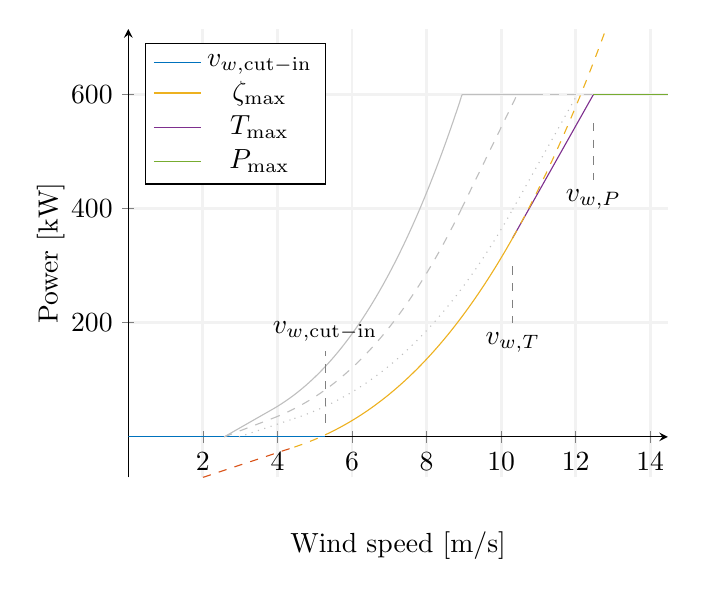
\begin{tikzpicture}
  \def\CL{2.1};
  \def\CDsys{0.18};
  \def\costheta{0.866};
  \def\etaairgrid{0.67};
  \def\Tmax{200};  % [kN]
  \def\Pmax{600};  % [kW]
  \def\Pgrav{50};  % [kW]
  \def\zetamax{(4/27 * \CL^3 / \CDsys^2)};
  \def\Ak{32.9};
  \def\rho{1.2};
  \def\vkitemin{30};
  \def\P0{(0.5 * \rho * \Ak * \CDsys * \vkitemin^3 / 1000)};
  \def\vcutin{(\CDsys / \CL * \vkitemin / \costheta)};
  \def\vT{((\Tmax * 1000 / 3 / (0.5 * \rho * \Ak * \zetamax))^0.5 / \costheta)};
  \def\vP{(\Pmax / (\etaairgrid * \Tmax * \costheta) + 2 * \vT / 3)};
  \def\vPtrue{(\vP + \Pgrav / (\etaairgrid * \costheta * \Tmax))};
  \def\vcutintrue{((1 + \Pgrav/(\etaairgrid * \P0)) * \vcutin)};
  \def\loydcoeff{(\etaairgrid * \costheta^3 * 0.5 * \rho * \Ak * \zetamax / 1000)};

\begin{axis}[axis lines=middle, samples=200,
    grid=both,
    grid style={line width=1pt, draw=gray!10},
    x label style={at={(axis description cs:0.5,-0.1)}, anchor=north},
    y label style={at={(axis description cs:-0.1,.5)}, rotate=90, anchor=south},
    xlabel={Wind speed [m/s]},
    ylabel={Power [kW]},
    legend pos=north west]
  \addplot[matlab1, domain=0:(\vcutintrue)] {0};
  %\addplot[matlab2, domain=(\vcutin):(1.5 * \vcutin)] {\etaairgrid * \P0 * (x / \vcutin - 1) - \Pgrav};
  \addplot[matlab3, domain=(\vcutintrue):(\vT)] {\loydcoeff * x^3 - \Pgrav};
  \addplot[matlab4, domain=(\vT):(\vPtrue)] {\etaairgrid * \costheta * \Tmax * (x - 2 * \vT / 3) - \Pgrav};
  \addplot[matlab5, domain=(\vPtrue):(\vPtrue + 2)] {\Pmax};
  \legend{$v_{\wind,\cutin}$, $\zeta_{\max}$, $T_{\max}$, $P_{\max}$};

  \addplot[matlab3, dashed, domain=(1.5 * \vcutin):(\vcutintrue)] {\loydcoeff * x^3 - \Pgrav};
  \addplot[matlab3, dashed, domain=(\vT):(\vT + 2.5)] {\loydcoeff * x^3 - \Pgrav};
  \addplot[matlab2, dashed, domain=2:(1.5 * \vcutin)] {\etaairgrid * \P0 * (x / \vcutin - 1) - \Pgrav};

  \def\costheta{1};
  \def\etaairgrid{1};
  \addplot[gray!50, domain=(\vcutin):(1.5 * \vcutin)] {\etaairgrid * \P0 * (x / \vcutin - 1)};
  \addplot[gray!50, domain=(1.5 * \vcutin):(\vT)] {\loydcoeff * x^3};
  \addplot[gray!50, domain=(\vT):(\vP)] {\etaairgrid * \costheta * \Tmax * (x - 2 * \vT / 3)};
  \addplot[gray!50, domain=(\vP):(\vP + 2)] {\Pmax};

  \def\costheta{1};
  \def\etaairgrid{0.67};
  \addplot[gray!50, dashed, domain=(\vcutin):(1.5 * \vcutin)] {\etaairgrid * \P0 * (x / \vcutin - 1)};
  \addplot[gray!50, dashed, domain=(1.5 * \vcutin):(\vT)] {\loydcoeff * x^3};
  \addplot[gray!50, dashed, domain=(\vT):(\vP)] {\etaairgrid * \costheta * \Tmax * (x - 2 * \vT / 3)};
  \addplot[gray!50, dashed, domain=(\vP):(\vP + 2)] {\Pmax};

  \def\costheta{0.866};
  \def\etaairgrid{0.67};
  \addplot[gray!50, dotted, domain=(\vcutin):(1.5 * \vcutin)] {\etaairgrid * \P0 * (x / \vcutin - 1)};
  \addplot[gray!50, dotted, domain=(1.5 * \vcutin):(\vT)] {\loydcoeff * x^3};
  \addplot[gray!50, dotted, domain=(\vT):(\vP)] {\etaairgrid * \costheta * \Tmax * (x - 2 * \vT / 3)};
%  \addplot[gray!50, dotted, domain=(\vP):(\vP + 2)] {\Pmax};

  \def\costheta{0.866};
  \def\etaairgrid{0.67};
  \draw[gray, dashed] (axis cs:{\vcutintrue}, 25) -- (axis cs:{\vcutintrue}, 150)
  node [above, black] {$v_{\wind,\cutin}$};
  %% \draw[gray, dashed] (axis cs:{1.5 * \vcutin}, 100) -- (axis cs:{1.5 * \vcutin}, 250)
  %% node [above, black] {$v_{\wind,v_{\kite}}$};
  \draw[gray, dashed] (axis cs:{\vT}, {\loydcoeff * \vT^3 - 100}) -- (axis cs:{\vT}, {\loydcoeff * \vT^3 / 2})
  node [below, black] {$v_{\wind,T}$};
  \draw[gray, dashed] (axis cs:{\vPtrue}, 550) -- (axis cs:{\vPtrue}, 450)
  node [below, black] {$v_{\wind,P}$};

\end{axis}
\end{tikzpicture}
\caption{Realistic power curve (colored) versus the ideal power curve
  (solid gray), power curve with conversion losses (dashed gray),
  power curve with conversion and off-downwind losses (dotted gray).
  This particular power curve assumes: $A_{\kite} = 32.9$ m$^2$,
  $v_{\kite,\min} = 30$ m/s, $\zeta_{\max} = 42.3$, $T_{\max} = 200$
  kN, $P_0 = 96$ kW, $P_{\max} = 600$ kW, $\theta = 30^{\circ}$,
  $\eta_{\airgrid} = 0.67$, and $P_{\grav} = 50$ kW.}
\end{center}
\end{figure}


\section{Mean power production}

The utility of a power curve is that it enables the calculation of the
mean power production, $\bar{P}$, at a site with a given wind
distribution.  The mean power production is found by integrating the
power curve weighted by the probability distribution function of the
wind speeds:
%
\begin{equation}
\bar{P} = \int_0^{v_{\wind,\cutout}} dv\, p(v) P(v)
\end{equation}

Assuming a Rayleigh distribution, Eq. \ref{eqn:rayleigh}, for the
distribution of wind speeds, it is possible to derive a closed form
solution for the mean power production of a kite system in terms of
the site's mean wind speed, $\bar{v}$, and the limits of the kite
system.
%
\begin{equation}
\label{eqn:rayleigh}
p(v) = \frac{\pi}{2} \frac{v}{\bar{v}^2} \exp \left(-\frac{\pi}{4} \frac{v^2}{\bar{v}^2} \right)
\end{equation}
%
The mean power is composed of terms from the Loyd-limited, tension
limited, and power limited sections of the power curve.
\begin{equation}
\bar{P} = \bar{P}_{\zeta} + \bar{P}_T + \bar{P}_P - \bar{P}_{\grav}
\end{equation}
%
Ignoring the gravity losses for now, the functional form of each of
these components is:
%
\begin{align}
\bar{P}_{\zeta} =&\;
\eta_{\airgrid} \cdot \frac{1}{2} \rho \zeta_{\max} \cos^3 \theta A \bar{v}^3 \\ \notag
&\times \left[\frac{6}{\pi} \erf \left(\frac{\sqrt{\pi}}{2} \frac{v_{\wind,T}}{\bar{v}}\right) -
\frac{v_{\wind,T}}{\bar{v}} \exp \left(-\frac{\pi}{4}\frac{v_{\wind,T}^2}{\bar{v}^2}\right)
\left(\frac{6}{\pi} + \frac{v_{\wind,T}^2}{\bar{v}^2}\right)
\right]
\end{align}

\begin{align}
\bar{P}_T =&\; \eta_{\airgrid} \cdot T_{\max} \cos \theta \bar{v} \\ \notag
           & \times \bigg[
\erf \left(\frac{\sqrt{\pi}}{2} \frac{v_{\wind,P}}{\bar{v}}\right) -
\erf \left(\frac{\sqrt{\pi}}{2} \frac{v_{\wind,T}}{\bar{v}}\right) \\ \notag
%
& \phantom{\times \bigg[} + \left(\frac{2}{3} \frac{v_{\wind,T}}{\bar{v}} -
\frac{v_{\wind,P}}{\bar{v}}\right)
\exp \left( -\frac{\pi}{4} \frac{v_{\wind,P}^2}{\bar{v}^2} \right) +
\frac{1}{3} \frac{v_{\wind,T}}{\bar{v}}
\exp \left( -\frac{\pi}{4} \frac{v_{\wind,T}^2}{\bar{v}^2} \right) \bigg]
\end{align}

\begin{equation}
\bar{P}_P = P_{\max} \exp \left( -\frac{\pi}{4} \frac{v_{\wind,P}^2}{\bar{v}^2}\right)
\end{equation}

\begin{equation}
  \bar{P}_{\grav} = P_{\grav} \left[
    \exp \left(-\frac{\pi}{4} \frac{v_{\wind,\cutin}^2}{\bar{v}^2} \right) -
    \exp \left(-\frac{\pi}{4} \frac{v_{\wind,P}^2}{\bar{v}^2} \right)
    \right]
\end{equation}

%% \subsection{Cost analysis}

%% In this simplified analysis, we assume some cost per unit power,
%% $c_P$, some cost per unit tension, $c_T$, and some cost per unit kite
%% area, $c_A$.

%% \begin{equation}
%% C = c_P P_{\max} + c_T T_{\max} + c_{\zeta A} \zeta A
%% \end{equation}

\section{Appendix}

\subsection{Gravity power loss}

Here is a sketch of the derivation of the velocity modulation for the
constant drag fraction strategy (see Eq. \ref{eqn:velocity_modulation}).

\begin{equation}
  m \dot v_{\kite} = m g_{\parallel} \cos \psi +
                     \frac{1}{2} \rho v_{\app} A (C_L v_{\wind} - C_D v_{\kite})
\end{equation}

\begin{equation}
  v_{\kite}(t) = v_{\kite, 0} + \delta v_{\kite}(t)
\end{equation}

Assuming $\delta v_{\kite}$ is small:
%
\begin{equation}
  m \delta \dot v_{\kite} = m g_{\parallel} \cos \psi -
                            \frac{1}{2} \rho v_{\kite, 0} C_D A \delta v_{\kite}
\end{equation}

\begin{align}
  \Delta v_{\kite} &= \int_{side}^{top} d \delta v_{\kite} \\
                   &= \int_0^{\pi/2} d\psi \frac{R_{\path}}{v_{\kite, 0}}
                      \left(g_{\parallel} \cos \psi -
                      \frac{1}{2} \rho \frac{v_{\kite, 0}}{m} A C_D \delta v_{\kite} \right)
\end{align}

\begin{equation}
  \frac{\Delta v}{v_{\kite,0}} \approx
  \frac{m g_{\parallel} R_{\path}}
       {m v_{\kite, 0}^2 +
        \frac{1}{2} \rho v_{\kite, 0}^2 A_{\kite} C_D R_{\path}}
\end{equation}


The time it takes to go around the loop is

\begin{equation}
  T_{\lp} = \int_0^{2 \pi} d\psi \frac{R}{v_{\kite,0} + \delta v}
          = \frac{R}{v_{\kite,0}} \int_0^{2 \pi} d\psi \frac{1}{1 + a \sin \psi}
          = \frac{T_{\lp,0}}{\sqrt{1 - a^2}}
\end{equation}
%
where $a = \Delta v / v_{\kite,0}$.

The energy made in a loop is

\begin{align}
  E_{\lp} &= \int_0^{2 \pi} d\psi R \frac{1}{2} \rho v_{\kite}^2 A_{\kite} \eta_{\airgrid} k C_{D_{\sys}} \\
          &= \int_0^{2 \pi} d\psi R \frac{1}{2} \rho v_{\kite,0}^2 (1 + a \sin \psi)^2 A_{\kite} \eta_{\airgrid}k C_{D_{\sys}} \\
          &= \frac{1}{2} \rho v_{\kite,0}^2 R A_{\kite} \eta_{\airgrid} k C_{D_{\sys}} \left(1 + \frac{a^2}{2} \right) 2 \pi
\end{align}

The power loss due to gravity may be found by comparing the $a=0$
power to the expected power.

\begin{align}
  P_{\grav} &= \frac{E_{\lp,0}}{T_{\lp,0}} - \frac{E_{\lp}}{T_{\lp}} \\
            &= P_0 \left( 1 - \sqrt{1 - a^2} - \frac{a^2}{2} \sqrt{1 - a^2} \right)
\end{align}

\end{document}
